\subsection{Research Method Extraction}
\label{section:research_method_extraction}
%\wo{Andrea ask for a structure. I suggest: Task (What to do), Challenges (Concrete Problem), Our Approach (Solution), Development of the controlled Vocabulary, Development of Training Corpus, Evaluation (if possible from Andreas introspection of SSOAR results, how good we solved the problem)}


\subsubsection{Task Description}
Inspired by a recent work of Nasar et al.
\cite{nasar2018information}, we define a list of basic entity types that give key-insights into scholarly publications. 
We adapted the list of semantic entity types to the domain of the social sciences with a focus on \textit{research methods},
but also including related entity types such as \textit{Theory, Model, Measurement, Tool, Performance}. We suspect that the division into semantic types might be helpful to find \textit{research methods}, because
related semantic entities types might provide clues or might be directly related to the research method itself.
For instance, in order to realize a certain research objective, an experiment is instrumented where a specific combination of \textit{methods} is applied to a \textit{data set} that might be intellectual or \textit{software}, thus achieving a specific \textit{performance} and result in that context.\\
%\\
\textbf{Example}: \textit{P-values} (measurement) are reported for the \textit{one-tail paired t-test} (method) on \textit{Allbus} (dataset) and \textit{ISSP} (dataset).\\


    %COMMENT (AZ): The following paragraph might be skipped
\paragraph{Formal problem definition}%\ \\[1pt]
Let $E$ denote a set of entities. The Named Entity Recognition and Linking task consists of (i) identifying entity mentions  $m$ in a sentence and, (ii) linking them, when possible, to a  reference knowledge base  $K$ (i.e, the SAGE Thesaurus\footnote{http://methods.sagepub.com}) 
and (iii) assigning a type to the entity, e.g., \textit{research method}, selected from a set of given types. 
Given a textual named entity mention $m$ along with the unstructured text in which it appears, the goal is to produce a mapping from the mention  $m$ to its referent real world entity  $e$ in  $K$.

\subsubsection{Challenges}
There are some major challenges that any named entity recognition, classification and linking system needs to handle.
First, regarding NER, identifying the entities boundary is important, thus detecting the exact sequence span. 
Second, ambiguity errors might arise in classification. For instance,`range' might be a domain-specific term from the knowledge base or belong to the general domain vocabulary. This is a challenging task for which context information is required. 
In the literature, this relates to the problem of \textbf{domain adaptation} which includes fine-tuning to specific named entity classes\footnote{apart from those used in traditional NER systems like \textit{Person}, \textit{Location}, or \textit{Organization} with abundant training data, as covered in the Stanford NER system\cite{finkel2005incorporating}}.
With respect to entity linking, another challenge is detecting name variations, since entities can be referred to in many different ways.
Semantically  similar words, synonyms or related words, which might be lexically or syntactically different, are often not listed in the knowledge base 
(e.g., the lack of certain terms like `questioning' but not `questionnaire').  This problem of automatically detecting these relationships is generally known as \textbf{linking problem}. 
Note that part of this problem also results from PDF-to-text conversion which is error-prone. 
Dealing with incomplete knowledge bases, i.e. \textbf{handling of out of vocabulary (OOV) items}, is also a major issue, since 
knowledge bases are often not exhaustive enough and do not cover specific terms or novel concepts from recent research.
Last but not least, the combination of different semantic types gives a more coherent picture of a research article. We hypothesize that such information would be helpful and results in an insightful co-occurrence statistics, and provides additional detail directly related to entity resolution, and finally helps to assess the \textbf{relevance of terms} by means of a score.

 
\subsubsection{Our Approach - Overview} 
Our context-aware framework builds on Stanford’s CoreNLP and Named Entity Recognition System\footnote{\url{https://nlp.stanford.edu/projects/project-ner.shtml}}. 
The information extraction process follows the workflow depicted in Figure~\ref{figure:pipeline}, using separate modules for pre-processing, classification, linking and term filtering.

We envision the task of finding entities in scientific publications as a sequence labeling problem, 
where each input word is classified as being of a dedicated semantic type or not.
In order to handle entities related to our domain, we train a novel machine learning classifier with major semantic classes,
%(see Table~\ref{tab:SemanticTypes}), 
using training material from the ACL RD-TEC 2.0 dataset  \cite{qasemizadeh2016acl}.
Apart from this, we follow a domain adaptation approach inspired by \cite{agerri2016robust} and ingest semantic background knowledge extracted from external scientific corpora, in particular the ACL Anthology~\cite{bird2008acl,gildea2018acl}.
We perform entity linking by means of a new gazetteer-based SAGE dictionary  of Social Research Methods  \cite{lewis2003sage}, thus putting a special emphasis on the social sciences. The linking component addresses the synonymy problem and matches an entity despite name variations such as spelling variations. 
Finally, term filtering is carried out based on a termhood and unithood, while scoring is achieved by calculating a relevance score based on TF-IDF (cf.  Section~\ref{para:relscore}).

%In order to conduct this study\dd{Study?}, 
Our research experiments are based on the repository for the Social Sciences SSOAR as well as the train and test data of the Rich Context Competition corpus\footnote{\url{https://coleridgeinitiative.org/richcontextcompetition}
with a total of 5,000 English documents}.
Our work extends previous work on this topic (cf. \cite{eckle2013automatically}) in various ways: First, we do not limit our study to abstracts, but use the entire fulltext. Second, we focus on a broader range of semantic classes, 
i.e. \textit{Research Method}, \textit{Research Theory}, \textit{Research Tool} and \textit{Research Measurement}, tackling also the problem of identifying novel entities.
 

\begin{figure}
\label{pipeline}
  \centering
    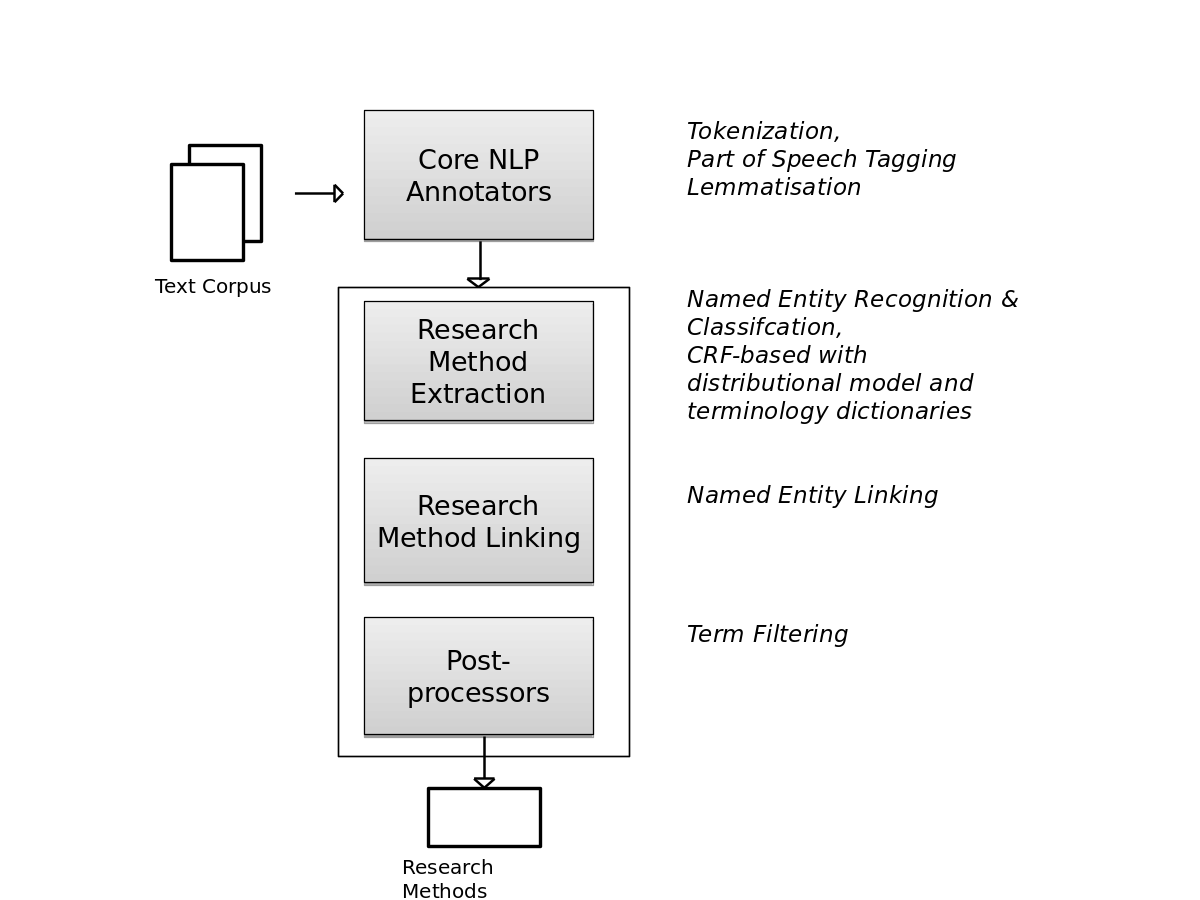
\includegraphics[width=0.47\textwidth]{figures/research-methods/pipeline.png}
    \caption{Overview of the entity extraction pipeline}
\end{figure}

\paragraph{Distributed Semantic Models}%\ \\[1pt]
\label{subsec:dist-model}
For domain adaptation, we integrate further background knowledge. We use vector embeddings  of words trained on additional corpora and which serve as input features to the CRF model. Semantic representations of words are a successful extension of common features, resulting in higher NER performance~\cite{Turian} and can be trained offline.


In this work, the word vectors were learned  from the scientific ACL ARC\footnote{\url{https://acl-arc.comp.nus.edu.sg/}} using Gensim with the skip gram model (cf. \cite{mikolov2013distributed}) 
and a pre-clustering algorithm\footnote{
Word embeddings are trained with a skip gram model using embedding size equal to 100, word window equal to 5, minimal occurrences of a word to be considered 10. Word embeddings are clustered using agglomerative clustering with a number of clusters set to {500,600,700} Ward linkage with euclidean distance is used to minimize the variance within the clusters.}. A summary of the size of the unlabeled  English data used for training word embeddings can be found in Table~\ref{tab:UnlabeledData}.

\begin{table}
\center
\small
  \caption{English data used for Training Word Embeddings}
  \label{tab:UnlabeledData}
  \begin{tabular}{lll}
    \toprule
    Corpus & Articles &  Documents/Tokens  \\
    \midrule
   ACL Corpus
    %ACL Anthology Reference Corpus
    &  22,878  &  806,791/2.5 GB \\ 
  \bottomrule
\end{tabular}
\end{table}

\paragraph{Features}%\ \\[1pt]
The  features incorporated into the linear chain CRF are shown in the Table~\ref{tab:features}. The features depend mainly on the observations  and  on  pairs  of  adjacent  labels, using a log-linear  combination. However, since simple token level training of CRFs leads to poor performance, more effective text features such as word shape, orthographic, gazetteer, Part-Of-Speech (POS) tags, along with word clustering (see Section~\ref{subsec:dist-model}) have been used.
%
\begin{table}
\small
  \caption{Features used for NER}
  \label{tab:features}
  \center
  \begin{tabular}{lc}
    \toprule
  \textbf{Type} &  \textbf{Features} \\
    \midrule
\textbf{Token unigrams} 	   &    $w_{i-2}$, $w_{i-1}$, $w_{i}$, $w_{i+1}$, $w_{i+2}$, ... \\

\textbf{POS unigrams} 	   &    $p_{i}$, $p_{i-1}$, $p_{i-2}$ \\

\textbf{Shapes}	   &    shape and capitalization \\
    \midrule
\textbf{NE-Tag}	   &    $t_{i-1}$, $t_{i-2}$ \\
      \midrule
\textbf{WordPair}	 &   
($p_{i}$, $w_{i}$, $c_{i}$) \\

\textbf{WordTag}	 &   
($w_{i}$, $c_{i}$) \\

    \midrule
\textbf{Gazetteer}	   &    SAGE gazetteer \\
    \midrule
    \textbf{Distributional Model}	   &    ACL Anthology model \\
      \bottomrule
   \end{tabular}
\end{table}

\paragraph{Knowledge Resources}%\ 
We use the SAGE thesaurus which includes well-defined concepts, an explicit taxonomic hierarchy between concepts as well as labels that specify synonyms of the same concept.
A portion of terms is unique to the social science domain (e.\,g.,  `dependent interviewing'), while others are drawn from related disciplines such as statistics (e.\,g., `conditional likelihood ratio test')\footnote{A glossary of statistical terms as provided in \url{https://www.statistics.com/resources/glossary/} has been added as well.}.
However, since the thesaurus is not exhaustive and covers only the top-level concepts related to social science methods, our aim was to extend it by automatically extracting further terms from domain-specific texts, in particular from the Social Science Open Access Repository.
More concretely, we carried out the following steps to extend SAGE as an off-line step. For step 2 and 3, candidate terms have been extracted by our pipeline for the entire SSOAR corpus. 
\begin{enumerate}
\item Assignment of semantic types to concepts (manual) 
\item Extracting terms variants such as abbreviations, synonyms, related terms from SSOAR (semi-automatic)
\item Computation of Term and Document Frequency Scores for SSOAR (automatic)
\end{enumerate}

\paragraph{Extracting term variants such as abbreviations, synonyms, and related terms}%\ \\[1pt]
26.082 candidate terms have been recognized and classified by our pipeline and manually inspected to  
a) find synonyms and related words that could be linked to SAGE, and
b) build a post-filter for incorrectly classified terms.  
Moreover, abbreviations have been extracted using the algorithm of Schwartz and Hearst
\cite{SchwartzH03}.
This way, a Named Entity gazetteer could be built and will be used at run-time. It comprises 1,111 terms from SAGE and 447 terms from the Statistics glossary as well as 54 previously unseen terms detected by the model-based classifier. 




\paragraph{Computation of Term and Document Frequency Scores}%\ \\[1pt]
Term frequency statistics have been calculated off-line for the entire SSOAR corpus.
The term frequency at corpus level will be used at run time to determine the term relevance at the document level by calculating the TF-IDF scores. The most relevant terms from SAGE are listed in Table~\ref{tab:SAGET}.
\begin{table}
\center
\small
  \caption{Most relevant terms from SAGE by Semantic Type}
\begin{tabular}{lll}
  \label{tab:SAGET}
  \textbf{SAGE Term} & \textbf{TF-IDF Score}  & \textbf{Semantic Class}   \\ \hline  
Fuzzy logic	  &	591,29  &		Research Method  \\
arts-based research	 &	547,21  &		Research Method \\
cognitive interviewing  &		521,13  &		Research Method \\  
QCA	 &	463,13  &		Research Method   \\ 
oral history	 &	399,68  &		Research Method \\ \hline  
market research  &		345,37  &		Research Field \\
life events  &		186,61  &		Research Field \\ \hline 
Realism  &		314,34  &		Research Theory \\
Marxism  &		206,77  &		Research Theory \\ \hline  
ATLAS.ti  &		544,51  &		Research Tool\\
GIS	 &	486,01  &		Research Tool\\
SPSS	  &	136,52  &		Research Tool \\ \hline  
  
\end{tabular}
\end{table}


\paragraph{Definition of a Relevance Score}%\ \\[1pt]
\label{para:relscore}
Relevance of terminology is often assessed using the notion of 
\textit{unithood}, i.e. `the degree of strength or stability of syntagmatic combinations of collections', and 
\textit{termhood}, i.e. `the degree that a linguistic unit is related to domain-specific concepts' \cite{kageura1996methods}.
Regarding \textit{unithood}, the NER model implicitly contains heuristics about legal POS tag sequences for candidate terms, 
consisting of at least one noun (NN), preceeded or followed by modifiers such as adjectives (JJ), participles (VB*) or cardinal numbers (CD), complemented by wordshape features.

In order to find out if the candidate term also fulfills the \textit{termhood} requirement, domain-specific term frequency statistics have been computed on the SSOAR repository, and set in contrast to general domain vocabulary terms. 
%\footnote{based on COCA, i.e. a large, balanced Corpus of Contemporary American English, using \textit{spoken, fiction, popular magazines and newspapers} rather than \textit{academic journals}, cf. \url{https://corpus.byu.edu/coca/} with frequency infos at \url{https://www.wordfrequency.info}}. 
It has to be noted  that only a small portion of the social science terms is actually unique to the domain (e.g.,  `dependent interviewing'), while others might be drawn from related disciplines such as statistics (e.g., `conditional likelihood ratio test').


%COMMENT (AZ) Since there is no gold standard it is difficult to report any reliable results! 
\paragraph{Preliminary Results}%\ \\[1pt]
Our method has been tested on 100 fulltext papers from SSOAR and 10 documents from the Rich Context Competition (RCC), all randomly selected from hold out corpora.
In our experiments on SSOAR Social Science publications, we compared results to the given metadata information.
The main finding was that while most entities from the SAGE thesaurus could be extracted and linked reliably (e.g., 'Paired t-test'), they could not be easily mapped to the SSOAR metadata terms, which consist of only a few abstract classes (e.g., 'quantitative analysis'). Furthermore, our tool was tested by the RCC organizer, were the judges reviewed 10 random publications and generated qualitative scores for each document.  %COMMENT (AZ) Yes. We were the winning team on this task. But what results to put here?

%COMMENT (AZ) Please double check 
%\subsubsection{Conclusion and Future Work}
%\label{subsec:ner-conclusion}
%A white paper describing our methods and approach will be published in a refereed special issue of the competition. 
%We plan to carry out a more detailed evaluation on fulltext scholarly publications and assess the impact of different features used in the ML model, including  background resources such as embeddings and dictionaries. 
